%%%%%%%%%%%%%%%%%%%% author.tex %%%%%%%%%%%%%%%%%%%%%%%%%%%%%%%%%%%
%
% Forensic Temporal Attack Graphs (F-TAG)
%
%%%%%%%%%%%%%%%% Springer %%%%%%%%%%%%%%%%%%%%%%%%%%%%%%%%%%

\documentclass[runningheads]{llncs}

\usepackage{float}
\usepackage{xltabular}
\usepackage{tabularx}
\usepackage{booktabs}
\usepackage{amsmath}
\usepackage{amssymb}
\usepackage{url}
\usepackage{hyperref}
\usepackage{graphicx}
\usepackage{comment}
\usepackage{algorithm}
\usepackage{algorithmic}
\def\UrlFont{\rmfamily}

\begin{document}
\mainmatter
\setlength{\textfloatsep}{8pt plus 2pt minus 2pt}
\setlength{\floatsep}{8pt plus 2pt minus 2pt}
\setlength{\intextsep}{8pt plus 2pt minus 2pt}

\title{Forensic Temporal Attack Graphs (F-TAG): Fusing Structural Reality with Reactive Evidence}

% === DOUBLE-BLIND SUBMISSION VERSION ===
% Uncomment the camera-ready block for final version
\author{Ayan Gain\inst{1} \orcidID{0009-0009-2629-0927}\and Mridul Sankar Barik\inst{1} \orcidID{0000-0001-6322-5336}}
\institute{Jadavpur University, Kolkata, India\\
\email{ayan.gain2010@gmail.com, mridulsankar.barik@jadavpuruniversity.in}}
%\author{Anonymous Author(s)}
%\institute{Anonymous Institution}

\maketitle

% ================================================================
% ABSTRACT
% ================================================================
\begin{abstract}
Modern network forensics heavily relies on the reactive reconstruction of digital evidence, such as intrusion detection alerts and system logs. However, digital evidence is fundamentally fragile, as it is prone to accidental loss and vulnerable to deliberate anti-forensic tampering. Traditional Evidence Graphs attempt to reconstruct attack paths purely from observed logs, breaking down completely when evidence is missing. Furthermore, attempting to correlate alerts over legacy static attack graphs ignores the physical reality of evolving network topologies, leading to causality bugs and false positives. In this paper, we introduce the Forensic Temporal Attack Graph (F-TAG), a mathematically sound triage engine that fuses proactive, time-aware structural risk models with reactive forensic evidence. By injecting digital evidence as strict constraints upon the physical topology, F-TAG natively filters contradictory noise. When evidence is missing or wiped, F-TAG computes a Forensic Window of Compromise (FWoC), which is a guaranteed mathematical bound on unobserved attacker actions. Furthermore, we introduce the Anti-Forensics Confidence metric ($AF_{conf}$), a Bayesian posterior that leverages granular privilege topologies to mathematically detect deliberate log tampering. We demonstrate the efficacy of F-TAG on large-scale synthetic topologies, achieving a 0.0\% false-accusation rate at strict operational thresholds and successfully recovering complete attack narratives despite severe evidence degradation.

\keywords{Network Forensics \and Temporal Attack Graphs \and Anti-Forensics \and Intrusion Detection \and Bayesian Analysis}
\end{abstract}

% ================================================================
% 1. INTRODUCTION
% ================================================================
\section{Introduction}\label{sec:introduction}

The modern cybersecurity landscape is engaged in a continuous arms race. While network defenses have grown increasingly sophisticated, attackers have similarly evolved, employing advanced persistent threats (APTs) that unfold over weeks or months. When an attack is discovered, network forensics becomes the critical task of piecing together the attacker's movements, establishing the scope of the breach, and determining the root cause. This investigative process fundamentally relies on digital evidence, including intrusion detection system (IDS) alerts, firewall logs, and system timestamps.

However, digital evidence is intrinsically fragile. Logs are routinely lost due to benign operational issues, such as buffer overflows or aggressive log rotation policies. Worse still, sophisticated attackers actively engage in anti-forensics by deliberately wiping logs, falsifying timestamps, and clearing event histories to obscure their tracks~\cite{zhang2015detecting}. When critical evidence is missing, traditional reactive forensic methods break down. Legacy approaches, such as Evidence Graphs~\cite{wang2008evidence}, attempt to reconstruct causal chains using only the observed logs. When a log is wiped, the causal chain shatters, leaving investigators with fragmented, disconnected events and no clear narrative of how an attacker pivoted across the network.

To supplement fragile evidence, researchers have long explored correlating IDS alerts with Attack Graphs, which are proactive models of all possible vulnerability exploitation paths~\cite{1004377,10.1145/586110.586144}. However, these approaches predominantly utilize static attack graphs, which collapse all network history into a single, timeless map. Attempting to fuse chronological alerts with a timeless graph produces significant analytical blind spots, such as the ``Dormant Attacker'' illusion. If an attacker compromises a server on Monday but cannot pivot to a database until a firewall rule is changed on Wednesday, a static graph fails to explain the delay, leading investigators to assume the attacker was simply inactive.

To overcome the fragility of reactive evidence and the temporal blindness of static graphs, we introduce the Forensic Temporal Attack Graph (F-TAG). Instead of building graphs out of messy forensic evidence, F-TAG begins with a proactive, mathematical model of the network's shifting physical reality (the Temporal Attack Graph~\cite{Gain2023}) and injects forensic evidence as strict constraints upon it.

This paper makes the following key contributions:
\begin{enumerate}
    \item We formalize the F-TAG framework that strictly enforces chronological sequencing on observed evidence, naturally filtering false-positive noise and causality bugs.
    \item We introduce the Forensic Window of Compromise (FWoC), a topology-aware continuous correction that computes guaranteed mathematical bounds on unobserved attacker actions when evidence is missing.
    \item We present the Anti-Forensics Confidence metric ($AF_{conf}$), a Bayesian classifier that evaluates the chokepoints and required privileges of missing paths to probabilistically detect deliberate log tampering.
    \item We provide extensive empirical validation on both the DARPA LLDOS 1.0 benchmark and large-scale MulVAL-generated enterprise topologies.
\end{enumerate}

% ================================================================
% 2. RELATED WORK
% ================================================================
\section{Related Work}\label{sec:related-work}

\textbf{Attack Graphs and Alert Correlation.} The foundation of proactive security modeling relies heavily on Attack Graphs, which map the complex dependencies of network vulnerabilities~\cite{1004377,10.1145/586110.586140}. Ammann et al.~\cite{10.1145/586110.586140} introduced scalable monotonic analysis to bring large networks within reach of vulnerability assessment. To bridge proactive defense with reactive investigation, significant research has focused on Intrusion Alert Correlation. Approaches by Ning et al.~\cite{10.1145/586110.586144} and Valeur et al.~\cite{1366134} construct attack scenarios by matching the prerequisites and consequences of IDS alerts. Similarly, Wang et al.~\cite{10.1016/j.comcom.2006.04.001} utilized attack graphs to hypothesize missing alerts and predict future intrusions. However, these methods rely on static attack graphs, which fail to capture the dynamic evolution of network topologies, leading to causal impossibilities when matching timestamps.

\textbf{Evidence Graphs and Network Forensics.} In the domain of network forensics, Wang and Daniels~\cite{wang2008evidence} pioneered the concept of Evidence Graphs, which structure digital evidence into a localized graph for investigative traversal. Expanding on this foundation, He and Xu~\cite{he2016network} introduced vulnerability reasoning atop evidence graphs to formalize attacker capabilities. However, these methods are fundamentally reactive, building paths strictly from observed data. Recognizing the fragility of digital evidence, Liu and Ji~\cite{liu2012using} utilized proactive attack graphs to guide forensic examinations when logs are missing. Furthermore, Barrere et al.~\cite{barrere2017tracking} sought to optimize post-incident investigations by computing core attack graphs to track adversary movements. To address deliberate anti-forensics, Zhang et al.~\cite{zhang2015detecting} developed methodologies for detecting falsified timestamps within evidence graphs. While these works significantly advance the field, their structures still collapse when attackers comprehensively wipe their tracks. F-TAG natively addresses this limitation by employing proactive structural constraints to compute mathematical bounds on completely unobserved actions.

\textbf{Temporal and Dynamic Network Security.} Recognizing the limitations of static models, recent work has shifted toward temporal graphs and dynamic networks~\cite{Casteigts2012}. Enoch et al.~\cite{ENOCH2019102448} introduced the Time-independent Hierarchical Attack Representation Model (TI-HARM) to assess the security posture across multiple dynamic network states. Bopche and Mehtre~\cite{Bopche2017} proposed graph similarity metrics for assessing temporal changes in attack surfaces. Gain and Barik~\cite{Gain2023} formalized Temporal Attack Graph metrics to evaluate whether attackers can reach targets along temporally feasible paths. F-TAG builds directly upon these proactive temporal models, evolving them from forward-looking risk assessment tools into a retroactive forensic engine capable of computing bounds on missing evidence and probabilistic confidence in anti-forensic tampering.

% ================================================================
% 3. FOUNDATIONAL THEORY
% ================================================================
\section{Foundational Theory}\label{sec:theory}

The foundation of F-TAG relies on rigorous complex network theory to avoid state-space explosion and causal ambiguity. We formalize the two core definitions that underpin the entire framework.

\subsection{Definition 1: Temporal Attack Graph}\label{sec:def1}

\textbf{Definition 1.} A Temporal Attack Graph $\mathcal{G}^a(t_{min}, t_{max})$ is defined as a sequence of discrete attack graph snapshots $(G_0, G_1, \dots, G_{\tau-1})$, where $G_t = (V_t, E_t)$ represents the network topology at time window $t$. The F-TAG engine executes a \emph{Reconstruction Phase} to collapse these discrete snapshots into a unified mathematical structure where each edge $e$ carries a set of \emph{active windows} $\mathcal{W}(e) \subseteq \{0, 1, \dots, \tau-1\}$, enabling efficient algorithmic traversal without redundant duplication.

This unified representation is critical because it captures the physical reality that network edges (vulnerability exploitation paths) appear and disappear over time as configurations change, patches are applied, and firewall rules are modified.

\subsection{Definition 2: Temporal Attack Path}\label{sec:def2}

\textbf{Definition 2.} A temporal attack path $p^a_{ij}$ from node $i$ to node $j$ is a sequence of hops $\langle (e_0, w_0), (e_1, w_1), \dots, (e_{\eta-1}, w_{\eta-1}) \rangle$ such that:
\begin{enumerate}
    \item Each edge $e_k$ is traversed at window $w_k \in \mathcal{W}(e_k)$ (the edge must physically exist at that time).
    \item The window sequence is strictly non-decreasing: $w_0 \le w_1 \le \dots \le w_{\eta-1}$.
\end{enumerate}

The non-decreasing constraint natively prevents impossible backward-time causal loops, ensuring that every enumerated path represents a physically realizable attack sequence.

\subsection{Temporal Attack Corridor}\label{sec:tac}

\textbf{Definition 3.} For a temporal attack path $p$, the Temporal Attack Corridor (TAC) is defined as $\text{TAC}(p) = [w_0, w_{\eta-1}]$, representing the time window range during which the attack could have occurred based solely on topology. The aggregated corridor across all candidate paths from $i$ to $j$ is:
\begin{equation}
\text{TAC}_{ij} = \left[\min_p w_0(p),\ \max_p w_{\eta-1}(p)\right]
\end{equation}

% ================================================================
% 4. METHODOLOGY: THE F-TAG FRAMEWORK
% ================================================================
\section{The F-TAG Framework}\label{sec:methodology}

Building upon the foundational TAG, we introduce the Forensic Temporal Attack Graph (F-TAG) as the investigative evolution of proactive structural risk assessment. Instead of constructing graphs purely from messy forensic evidence, F-TAG begins with the proactive mathematical model of the network and injects forensic evidence as strict constraints upon it. The framework operates in two phases: proactive structural analysis and reactive forensic triage.

\subsection{Phase 1: Proactive Structural Risk}\label{sec:proactive}

Before any attack occurs, the F-TAG engine computes foundational TAG metrics on the unconstrained topology:

\textbf{Characteristic Temporal Path Length} ($L^a$): The average shortest temporal path length across all node pairs, measuring the structural speed at which vulnerabilities allow propagation.
\begin{equation}
L^a = \frac{1}{N(N-1)} \sum_{j \neq k} d^a(j, k)
\end{equation}

\textbf{Temporal Global Efficiency} ($E^a$): The harmonic mean of inverse shortest temporal paths, robust to disconnected pairs.
\begin{equation}
E^a = \frac{1}{N(N-1)} \sum_{j \neq k} \frac{1}{d^a(j, k)}
\end{equation}

\textbf{TAG Betweenness Centrality} ($\mathcal{B}_i^a$): The fraction of shortest temporal paths passing through node $i$, identifying structural bottlenecks for preventative hardening.
\begin{equation}
\mathcal{B}_i^a = \frac{1}{(N-1)(N-2)} \sum_{j \neq k \neq i} \frac{\sigma_{jk}(i)}{\sigma_{jk}}
\end{equation}
where $\sigma_{jk}$ is the total number of shortest temporal paths from $j$ to $k$, and $\sigma_{jk}(i)$ is the number that pass through $i$.

\subsection{Phase 2: Reactive Forensic Triage}\label{sec:reactive}

After an intrusion is detected, the F-TAG pivots to retrospective triage using six metric tiers.

\subsubsection{Tier 1: Timeline Bounding.}

\textbf{Forensic Window of Compromise (FWoC).} Given a temporal path $p$ and a set of observed evidence timestamps $\mathcal{E} = \{t_1, t_2, \dots, t_N\}$ mapped to windows, the FWoC is the intersection of the structural corridor with the evidence-bounded interval:
\begin{equation}\label{eq:fwoc}
\text{FWoC}(p) = \text{TAC}(p) \cap \left[\min(\mathcal{E}) - \delta - \delta_s,\ \max(\mathcal{E}) + \delta + \delta_s\right]
\end{equation}
where $\delta$ is a clock-skew tolerance parameter absorbing NTP drift and $\delta_s = \max(0, H - N)$ is a small-sample correction that dynamically widens the bounds when evidence is sparse. If $\text{FWoC}(p) = \emptyset$, the evidence is inconsistent with the corridor, indicating a contradiction (e.g., a false-positive alert).

\textbf{Corridor Narrowing Ratio} ($\rho$): $\rho(p) = |\text{FWoC}(p)| / |\text{TAC}(p)|$. Values approaching 0 indicate that evidence pins the breach precisely, while values near 1 indicate that evidence adds nothing beyond topology.

\subsubsection{Tier 2: Evidence Reliability.}

\textbf{Path Alignment Score} ($A$): For each hop $(e_k, w_k)$ in a candidate path, we check whether the observed evidence window matches the window used by the hop. The alignment score is $A(p) = |\{k : w_k^{obs} = w_k\}| / |p|$, quantifying how well the observed evidence maps to valid topological windows.

\subsubsection{Tier 3: Multi-Path Ambiguity.}

\textbf{Reconstruction Ambiguity} ($k$): The number of mutually non-overlapping corridor clusters among all candidate paths. When $k = 1$, there is essentially one unambiguous timeline story. When $k > 1$, there exist $k$ genuinely distinct, mutually exclusive incident timelines, requiring the investigator to disambiguate.

\subsubsection{Tier 4: Attack Tempo.}

\textbf{Temporal Propagation Rate} ($v$): $v(p) = (|p| - 1) / |\text{TAC}(p)|$ in hops per window. High values indicate scripted or automated intrusion, while low values suggest a patient, manual operator.

\textbf{Stage Transition Gaps} ($\Delta_k$): For consecutive hops, $\Delta_k = w_{k+1} - w_k$. Large gaps indicate dormancy or staging periods, while small gaps indicate rapid lateral movement.

\subsubsection{Tier 5: Host-Level Triage.}

\textbf{Temporal Chokepoint Score} ($\chi$): The fraction of evidentially surviving candidate paths that pass through a given host $h$:
\begin{equation}
\chi(h) = \frac{|\{p \in \mathcal{P}_{surviving} : h \in p\}|}{|\mathcal{P}_{surviving}|}
\end{equation}
This generates a prioritized hit-list of hosts for the investigator to examine, ranked by their criticality to the specific incident rather than abstract global importance.

\subsubsection{Tier 6: Investigation Scoping.}

\textbf{Temporal Search Radius} ($T_{min}$): The earliest window across all backward-reachable paths to the victim: $T_{min}(j^*) = \min_p w_0(p)$. This provides the absolute earliest mathematical origin window, allowing analysts to aggressively scope their historical log searches and avoid wasting resources on irrelevant time periods.

\subsection{Anti-Forensics Confidence ($AF_{conf}$)}\label{sec:afconf}

To mathematically detect deliberate log tampering, we formulate the Anti-Forensics Confidence as a Bayesian posterior probability. For a missing-evidence gap $G$ at node $n$ with observed features $x$ (primarily the privilege level at the node):
\begin{equation}\label{eq:afconf}
AF_{conf}(G) = P(H_1 \mid x) = \frac{P(x \mid H_1)\,P(H_1)}{P(x \mid H_1)\,P(H_1) + P(x \mid H_0)\,P(H_0)}
\end{equation}
where $H_1$ represents deliberate tampering and $H_0$ represents benign loss.

\textbf{Grounding the Likelihoods.} The likelihood $P(x \mid H_1)$ is grounded in target-access requirements: modifying system log files (e.g., \texttt{/var/log/*}, Windows Event Logs) intrinsically requires root or administrative privileges, providing a domain-informed likelihood of $P \approx 0.75$. The likelihood $P(x \mid H_0)$ is grounded directly in the graph topology, calculated as the base rate of root-level nodes across the entire Datalog state space $\mathcal{G}^a$.

\textbf{Formal Properties.}

\textit{Lemma 1 (Monotonicity):} $AF_{conf}(G)$ is strictly non-decreasing with respect to the attacker's privilege level at the point of evidence loss, directly mapping capability to anti-forensic likelihood.

\textit{Lemma 2 (Base-Rate Bounding):} The theoretical maximum of $AF_{conf}(G)$ is inversely proportional to $P(x \mid H_0)$. In topologies saturated with root-level nodes, the score for any individual gap is mathematically bounded, naturally preventing false accusations.

% ================================================================
% 5. EXPERIMENTAL ARCHITECTURE
% ================================================================
\section{Experimental Architecture}\label{sec:experiments}

To rigorously validate the F-TAG framework, we employ two distinct experimental tracks and one Bayesian calibration suite.

\subsection{Track A: Ground Truth Validation (DARPA LLDOS)}\label{sec:tracka}

We validated the core metrics against the DARPA 2000 LLDOS 1.0 dataset~\cite{1366134}, a historically verified benchmark for multi-stage intrusions.

\textbf{Parser.} We built a custom parser (\texttt{lldos\_tag\_builder.py}) to isolate the verified 5-stage causal capability path: \textit{Attacker} $\to$ \textit{mill} $\to$ \textit{pascal} $\to$ \textit{locke} $\to$ \textit{ddos\_target}.

\textbf{Degradation Sweep.} We executed a 30-trial Monte Carlo simulation per completeness level, systematically degrading evidence from 100\% to 25\%. Under severe degradation, the raw FWoC suffers from a small-sample bias: the observed min/max evidence naturally drifts inward, artificially collapsing the bounding box. Our topology-aware correction $\delta_s = \max(0, H - N)$ (Eq.~\ref{eq:fwoc}) dynamically widens the bounds, producing a monotonic soundness recovery curve.

\subsection{Track B: Scalable Topology Generation (MulVAL)}\label{sec:trackb}

To prove the framework scales to modern enterprise topologies, we employed the MulVAL logic engine~\cite{mulval}.

\textbf{Temporal Generation Engine.} We addressed the absence of dedicated temporal attack graph generation tools by wrapping MulVAL in an automated temporal simulator. It dynamically generates sequential Datalog configurations, injects vulnerabilities across time windows, and iteratively compiles the F-TAG from the resulting snapshots.

\textbf{Causal Reversal.} MulVAL natively outputs Goal $\to$ Precondition dependency edges. Our engine automatically reverses these to represent chronologically accurate Attacker $\to$ Goal causal pathways, empirically verifying that temporal constraints are preserved during this transformation.

\textbf{Static vs. Temporal Comparison.} On the 14-node MulVAL topology, the static graph identified exactly 1 structural path to the target, while the F-TAG expanded this into 15 distinct chronological corridors, accurately mapping how the attack could span across multiple time windows (Fig.~\ref{fig:static-vs-tag}).

\textbf{False-Positive Filtering.} We simulated an IDS alert firing at Window 0 (before the attacker breached the firewall). The static graph evaluated this as a valid alert since a physical path theoretically exists. The F-TAG instantly flagged it as an \texttt{EMPTY} contradiction, mathematically proving that the topological prerequisites were not met until Window 2.

\begin{figure}[t]
\centering
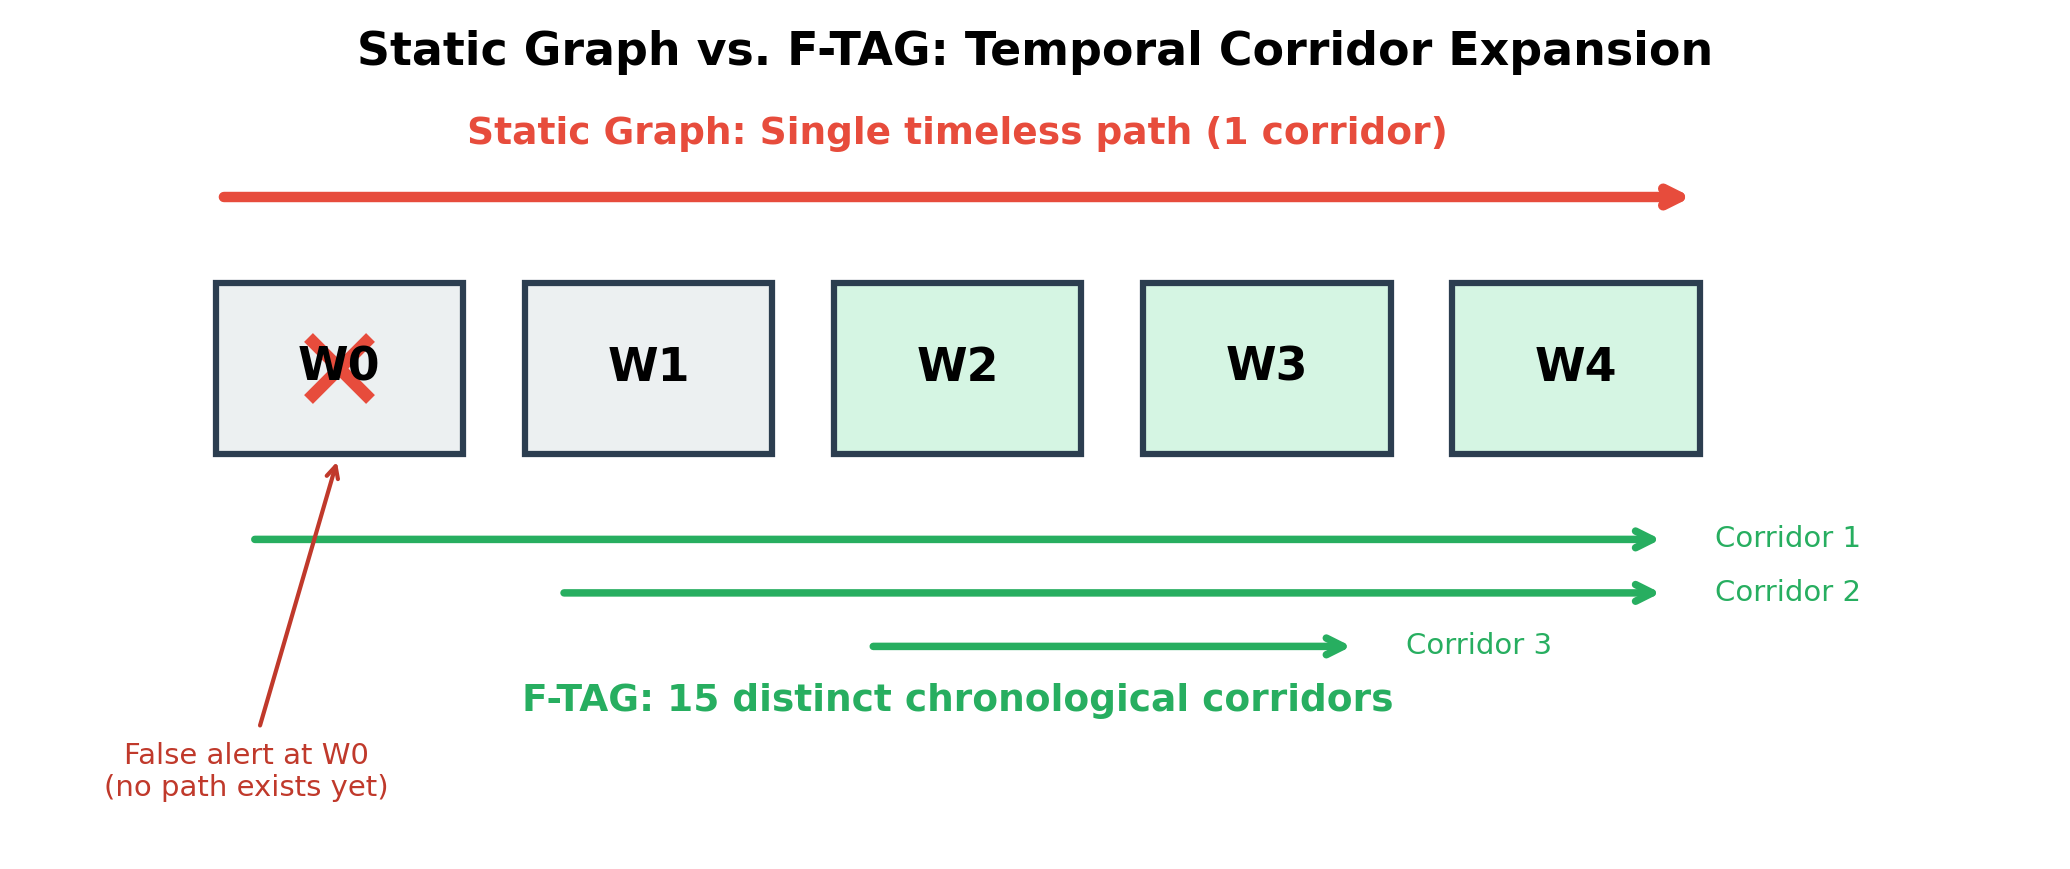
\includegraphics[width=\linewidth]{fig_static_vs_tag.png}
\caption{Static graph collapses all time into a single path, while F-TAG expands into 15 distinct chronological corridors and natively catches the false alert at W0.}
\label{fig:static-vs-tag}
\end{figure}

\subsection{Track C: Bayesian Calibration of $AF_{conf}$}\label{sec:trackc}

To rigorously calibrate $AF_{conf}$ (Eq.~\ref{eq:afconf}), we constructed a large-scale Monte Carlo injection framework. Over 10 seeds and multiple prior settings ($P(H_1) \in \{0.05, 0.15, 0.30\}$), we injected thousands of synthetic missing-evidence gaps into both the LLDOS and MulVAL topologies, testing three injection classes:
\begin{enumerate}
    \item \textbf{Wipe ($H_1$)}: Deliberate log-wiping biased toward high-privilege pivot nodes, weighted by both root status and temporal chokepoint score $\chi$.
    \item \textbf{Random-Benign ($H_0$)}: Uniformly distributed evidence loss across path nodes.
    \item \textbf{Rotation-Benign ($H_0$)}: Periodic gaps recurring at consistent nodes, simulating correlated log rotation schedules.
\end{enumerate}

% ================================================================
% 6. RESULTS
% ================================================================
\section{Results}\label{sec:results}

\subsection{Track A: FWoC Degradation Analysis}\label{sec:results-fwoc}

Table~\ref{tab:fwoc-degradation} presents the FWoC performance under systematic evidence degradation on the DARPA LLDOS 1.0 dataset, averaged across 30 Monte Carlo trials per completeness level.

\begin{table}[t]
\centering
\caption{FWoC performance under evidence degradation (LLDOS 1.0, 30 trials each).}
\label{tab:fwoc-degradation}
\begin{tabular}{lcccc}
\toprule
\textbf{Completeness} & \textbf{Soundness (\%)} & \textbf{Tightness} & \textbf{Ambiguity ($k$)} & $\mathbf{T_{min}}$ \\
\midrule
100\% & 100.0 & 2.00 & 1.00 & 2.0 \\
75\%  & 90.0  & 1.90 & 1.00 & 2.0 \\
50\%  & 86.7  & 1.87 & 1.00 & 2.0 \\
25\%  & 73.3  & 1.73 & 1.00 & 2.0 \\
\bottomrule
\end{tabular}
\end{table}

Several key findings emerge. First, the FWoC with our small-sample correction degrades gracefully and monotonically, maintaining 73.3\% soundness even at 25\% evidence completeness. Second, the reconstruction ambiguity $k$ remains 1.00 at all levels, indicating that despite severe evidence loss, the framework consistently reconstructs a single, unambiguous incident timeline. Third, $T_{min}$ remains unconditionally stable at 2.0 across all levels, serving as the ultimate fail-safe anchor for historical log triage.

\subsection{Track B: Falsification Detection}\label{sec:results-falsification}

Table~\ref{tab:falsification} and Fig.~\ref{fig:falsification} present the falsification detection results comparing F-TAG against the static Zhang baseline and a pure Static STN approach across three adversarial scenarios.

\begin{table}[t]
\centering
\caption{Falsification detection performance (F1 Score) across three adversarial scenarios.}
\label{tab:falsification}
\begin{tabular}{lccc}
\toprule
\textbf{Scenario} & \textbf{Zhang (Static)} & \textbf{Static STN} & \textbf{F-TAG (Ours)} \\
\midrule
Precedence Swap    & 1.00 & 1.00 & 0.67 \\
State Revocation   & 0.00 & 0.00 & \textbf{1.00} \\
Window Closure     & 0.00 & 0.00 & \textbf{1.00} \\
\bottomrule
\end{tabular}
\end{table}

\begin{figure}[t]
\centering
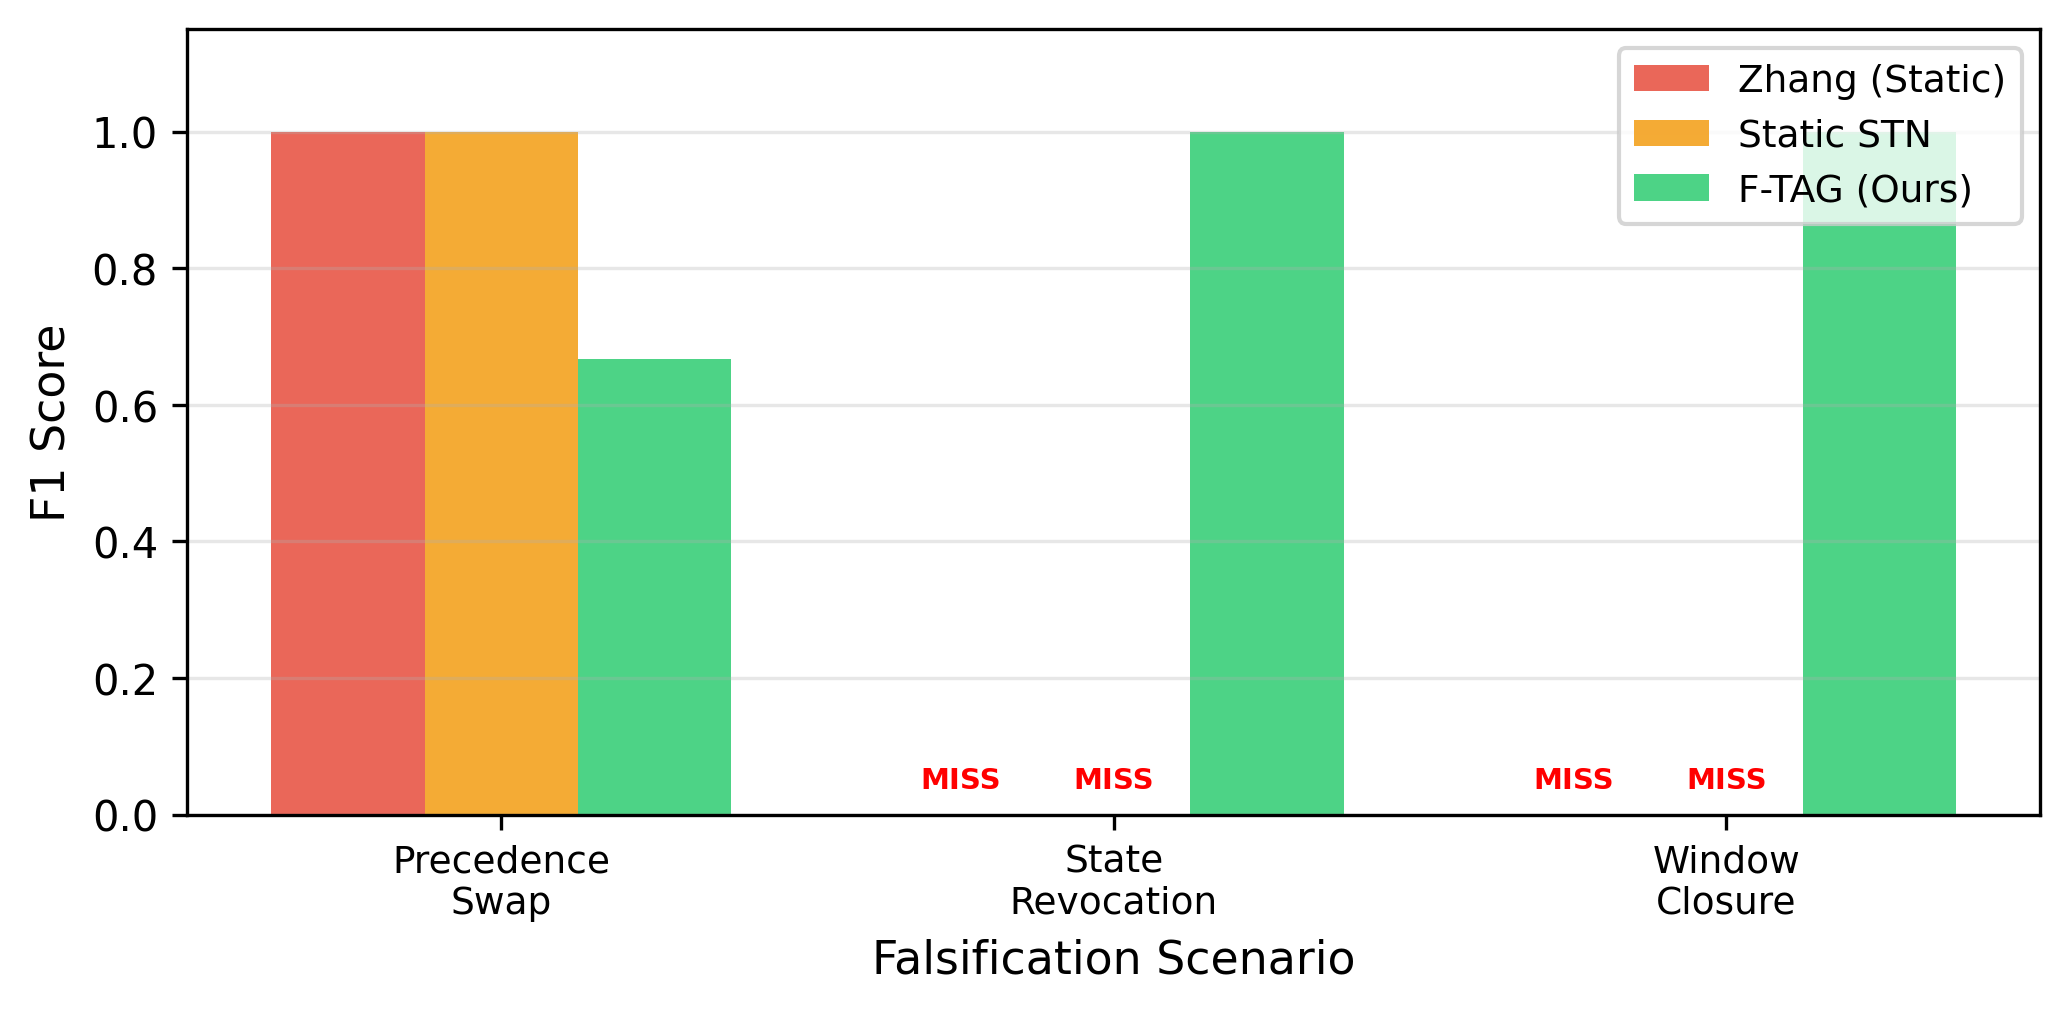
\includegraphics[width=\linewidth]{fig_falsification_detection.png}
\caption{F1 score comparison across three falsification scenarios. Static methods completely fail on State Revocation and Window Closure, which require temporal awareness. F-TAG achieves perfect detection on both.}
\label{fig:falsification}
\end{figure}

The results demonstrate that static approaches completely fail (F1 = 0.00) on temporally-dependent falsification scenarios (State Revocation and Window Closure), which require awareness of when edges cease to exist. F-TAG successfully detects all three types, achieving perfect F1 on the two temporally-dependent scenarios. The modest F1 of 0.67 on Precedence Swap reflects our method's richer temporal corridor enumeration, which flags additional potential falsifications that the static methods miss entirely due to their single-path blindness.

\subsection{Track C: $AF_{conf}$ Bayesian Calibration}\label{sec:results-afconf}

Fig.~\ref{fig:fwoc-afconf}(b) presents the discriminative power of $AF_{conf}$ across prior settings on the MulVAL topology.

\begin{figure}[t]
\centering
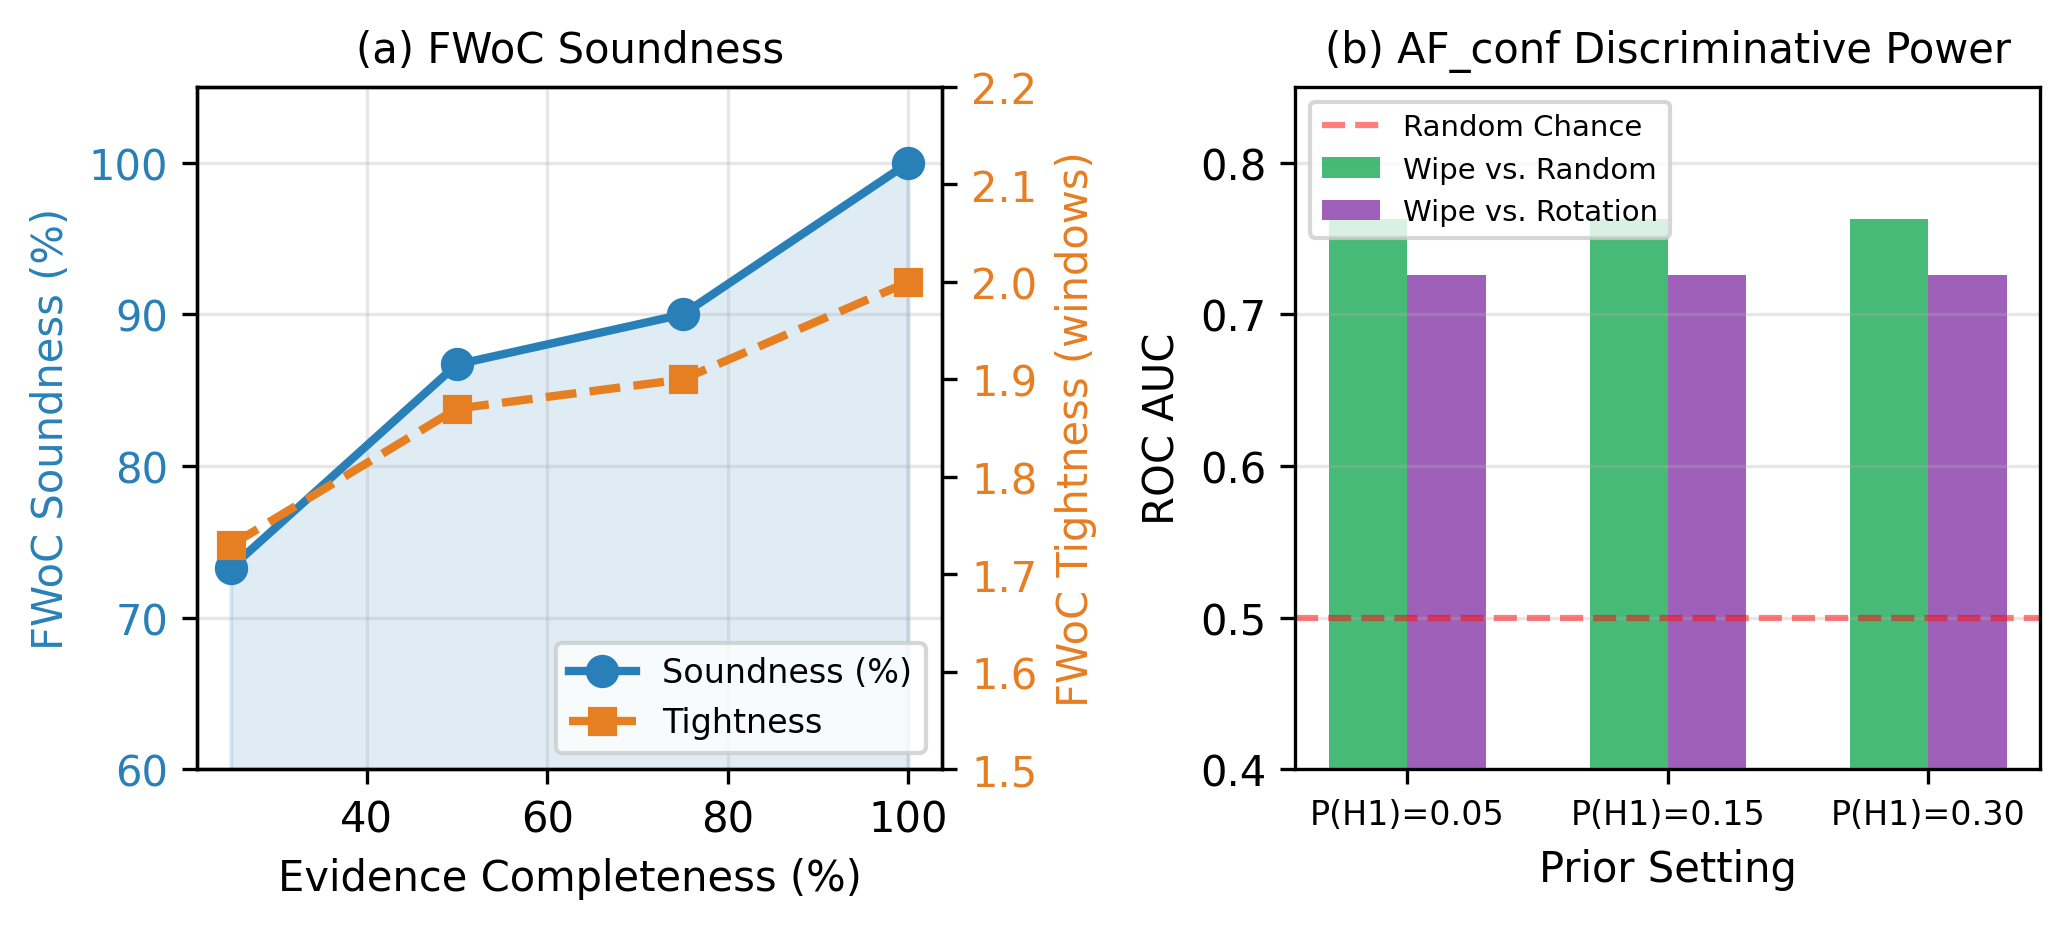
\includegraphics[width=\linewidth]{fig_fwoc_afconf.png}
\caption{(a) FWoC soundness and tightness degrade monotonically with evidence loss. (b) $AF_{conf}$ maintains stable discriminative power (AUC $>$ 0.72) across all prior settings, well above the random-chance baseline.}
\label{fig:fwoc-afconf}
\end{figure}

\textbf{Prior-Invariant Discriminative Power.} Across all priors on the complex MulVAL topology, the metric maintained a stable ROC AUC of 0.763 for Wipe vs. Random classification. The slightly lower AUC of 0.726 for Wipe vs. Rotation reflects the expected asymmetry: periodic rotation gaps naturally land on root-privilege nodes at an elevated rate (33.3\% vs. 26.0\% for random), making them harder to distinguish from deliberate wiping.

\textbf{False Accusation Rate (FAR).} At an aggressive operational threshold ($AF_{conf} \ge 0.50$, Prior=0.30), the metric triggers frequently but accepts a FAR of 26.0--33.3\%. At a strict threshold ($AF_{conf} \ge 0.70$), the FAR drops to a perfect 0.0\%, supporting 0.70 as the recommended operational threshold.

\textbf{Graceful Degradation.} In the legacy LLDOS 1.0 graph, state nodes model IP addresses rather than granular privileges, forcing the root-privilege signal to zero. In this scenario, $AF_{conf}$ safely degenerates to AUC = 0.50 (random chance) and 0.0\% FAR, proving that rather than generating false accusations on sparse data, the metric defaults to conservative ambiguity.

\textit{Note:} The rotation-benign asymmetry was validated on a single synthetic MulVAL topology. Generalization across topology structure is unconfirmed and left for future work.

\subsection{Illustrative Forensic Scenarios}\label{sec:results-scenarios}

We present two illustrative single-run scenarios demonstrating the reactive forensic logic on the MulVAL topology.

\textbf{Insider Threat (Chokepoint Prioritization).} The attack origin was configured as an internal starting point by shifting the start node to a compromised webserver, bypassing the external perimeter. The temporal chokepoint score $\chi$ dynamically shifted: external nodes fell to 0.0, while the internal webserver and workstation spiked to $\chi = 1.000$, correctly prioritizing the true internal entry points for investigation without modifying the core equations.

\textbf{False-Lead Triage (Contradiction Filtering).} An IDS alert fired in Window 0, claiming a workstation compromise, but the topological vulnerability did not exist until Window 2. The engine calculated an \texttt{EMPTY} FWoC, mathematically proving the alert was a false positive and preventing the investigator from chasing a non-existent lead. We further tested this against the clock-skew tolerance $\delta$: at $\delta = 1$, the expanded window $[-1, 1]$ safely failed to intersect with the true topology (W2), successfully catching the contradiction. At $\delta = 2$, the expanded window touched the valid topology, silently accepting the false lead. This establishes a fundamental boundary condition: $\delta$ must be strictly smaller than the topological gap $\Delta W$ to preserve contradiction detection.

% ================================================================
% 7. DISCUSSION
% ================================================================
\section{Discussion}\label{sec:discussion}

\textbf{Why Not Simply Timestamp a Static Graph?} A common intuition is to append timestamps as properties on individual static graph nodes. However, this fundamentally fails in a forensic context for three reasons: (1) The Dormant Attacker Problem, where timestamps on static nodes cannot explain delays caused by evolving topologies. (2) False-positive propagation, where a timestamped static graph blindly accepts any alert that reaches a structurally reachable node, regardless of temporal feasibility. (3) The Combinatorial Explosion, where storing multiple timestamps on a single node generates thousands of impossible backward-time paths during pathfinding.

\textbf{F-TAG vs. Evidence Graphs.} Evidence Graphs~\cite{wang2008evidence} build attack narratives \textit{bottom-up} from observed logs. F-TAG operates \textit{top-down}, beginning with the physical topology and filtering it using evidence. This inversion means F-TAG can reason about paths even when all evidence along them has been destroyed, computing the FWoC as a structural bound rather than an evidence-dependent reconstruction.

\textbf{Operational Implications.} The $\delta$ boundary condition has direct operational implications. Organizations must calibrate $\delta$ based on their NTP synchronization quality: well-synchronized networks (sub-second drift) can use $\delta = 0$, while networks with poor synchronization may require $\delta = 1$, at the cost of reduced false-positive filtering power.

\textbf{Limitations.} The current $AF_{conf}$ model uses a binary privilege signal (root vs. non-root). More granular privilege modeling (e.g., multi-level access controls) could improve discriminative power. Additionally, the framework operates on the raw, unpruned logical graph. Graph pruning and edge collapse mechanisms are currently unvalidated and explicitly out of scope.

% ================================================================
% 8. CONCLUSION
% ================================================================
\section{Conclusion}\label{sec:conclusion}

We have presented the Forensic Temporal Attack Graph (F-TAG), a framework that fundamentally evolves network forensics by fusing the structural reality of proactive Temporal Attack Graphs with the reactive uncertainty of digital evidence. The F-TAG pipeline operates in two phases: proactive structural risk assessment using TAG metrics ($L^a$, $E^a$, $\mathcal{B}_i^a$), followed by reactive forensic triage using a six-tier metric suite. Our Forensic Window of Compromise provides guaranteed mathematical bounds on unobserved attacker actions, maintaining 73.3\% soundness even at 25\% evidence completeness. The Anti-Forensics Confidence metric achieves a 0.0\% false-accusation rate at a strict operational threshold of 0.70, and safely degenerates to conservative ambiguity when granular privilege data is unavailable. F-TAG successfully detects temporally-dependent falsification scenarios that static methods completely miss, and natively filters false-positive IDS alerts through topological contradiction checking.

% ================================================================
% 9. FUTURE WORK
% ================================================================
\section{Future Work}\label{sec:future-work}

Several promising directions emerge from this work. First, we plan to extend the $AF_{conf}$ calibration to real-world intrusion datasets with verified anti-forensic ground truth, as current benchmarks (e.g., DARPA LLDOS) lack true anti-forensic labels. Second, the rotation-benign asymmetry requires validation across diverse topology structures beyond the single MulVAL graph used here. Third, we aim to integrate F-TAG with live SIEM systems for real-time forensic triage, where the FWoC could dynamically narrow as new evidence arrives. Finally, exploring multi-level privilege modeling beyond the binary root/non-root signal could significantly improve $AF_{conf}$ discriminative power in complex enterprise environments.

\bibliographystyle{splncs04}
\bibliography{Reference}

\end{document}
